    \chapter{Methods}

    The methods utilized in this work are presented in the following chapter. This includes introductions into Bayesian analysis and decision theory. In particular Bayesian inference, estimation of uncertain values and how loss function can be used in this context. These methods are incorporated in the context of numerical modeling of structural geological settings. This is done by programming in a python environment. Central tools for model construction and conduction of the statistical evaluation are Geomodeler3D, GemPy and PyMC in particular and are also presented in this chapter.
    
        \section{Bayesian analysis and decision theory}
	    Problems and reasoning behind decision making are examined in the field of decision theory, as implied by the name \cite{berger2013stat}. Such decision problems are commonly influenced by parameters that are uncertain. In statistical decision theory, the presence of statistical knowledge is used to gain information on the nature of these uncertainties. (Such uncertain parameters can be considered as numerical quantities.) In order to find the best decision to a problem, it is possible to combine sample information with other aspects such as the possible consequences of decision making and the availability of prior information on our uncertainties. Decision consequences are expressed as gains in economic decision theory and as losses, which equal negative gains, in statistics. Prior information might be given for example due to experience from previous similar problems or from expert knowledge (see Batvold and Begg). The approach of utilizing such as priors is known as Bayesian analysis and is explained in the following \cite{berger2013stat}. (It goes well with decision theory.)
	    
	    \section{Basic elements}
	    Some basic elements are to be defined. The unknown (uncertain?) quantity influencing decision making is usually named denominated as $\theta$, the state of nature. Given statistical information on $\theta$ in the form of probability distributions, $\theta$ is called the parameter. 
	    Decisions are also referred to as actions $a$.
	    The outcome of statistical tests in form of information or statistical evidence is denoted as $X$.	    
	    Loss is defined as $L(\theta,a)$, so $L(\theta_1,a-1)$ is the actual loss incurred when action $a_1$ is taken while the true state of nature is $\theta_1$ \cite{berger2013stat}. Loss, expected loss and loss functions are further explained below.  
        
        \subsection{Bayesian inference}
        Bayesian inference is most importantly characterized by its preservation of uncertainty, in contrast to standard statistical inference \cite{davidson2015}. Probability is seen as a measure of belief for an event to occur. It has been argued by \cite{davidson2015}  that this Bayesian approach is intuitive and inherent in the natural human perspective. These beliefs can furthermore be assigned to individuals \cite{davidson2015}. Thus, different and even contradicting beliefs about the probability of an event might be held by different individuals, based on variations and disparities in the information available to each one individual \cite{davidson2015}.
        The initial belief or guess about an event A can be denoted as P(A). This is used as the so-called prior probability on which Bayesian updating is based. The beliefs about the occurrence of an event are revalued in the presence of additional information, i.e. the observation of new evidence which can be denominated as X. These observations are included as likelihoods P(X$|$A). This process of updating results in a posterior probability P(A$|$X) \cite{davidson2015}. It is important to note that the prior is not simply discarded but re-weighted by Bayesian updating. It was also pointed out by \cite{davidson2015} that by utilizing an uncertain prior, the potential for wrongfulness of the initial guess is already included. This means that Bayesian updating is about reducing uncertainty in a belief and reaching a guess that is less wrong \cite{davidson2015}.
        Bayesian updating is defined by and conducted via the following equation, called the Bayes' Theorem:
        
        \begin{equation}\label{eq:BayesTheorem}
        P(A|X) = \frac{P(X|A)P(A)}{P(X)}
        \propto P(X|A)P(A)
        \end{equation}
        
        -Law of Large Numbers!
               
        \subsection{Estimation}
        The resulting posterior distribution can be used to acquire point estimates for the true state of nature $\theta$. Common and simple examples for such estimators are the mode (i.e. the generalized maximum likelihood estimate), the mean and the median of a distribution \cite{berger2013stat}. The presentation of a point estimate should usually come with a measure for its estimation error. According to \cite{berger2013stat}, the posterior variance is most commonly used as an indication for estimate accuracy. However, it is argued by \cite{davidson2015} that by using pure accuracy metrics, while this technique is objective, it ignores the original intention of conducting the statistical inference in cases, in which payoffs of decisions are valued more than their accuracies. A more appropriate approach can be seen in the introduction of loss and the use of loss functions \cite{davidson2015}.
        
        \subsection{Expected loss and loss functions} 
        Loss is a statistical measure of how bad an estimate is, i.e. how much is lost by making a certain decision. Gains are considered by statisticians as negative losses \cite{davidson2015}.
        The magnitude of an estimate's loss is defined by a loss function, which is a function of the estimate of the parameter and the true value of the parameter \cite{davidson2015}:
        
        \begin{equation}\label{eq:LossFunction}
        L(\theta,\hat{\theta}) = f(\theta,\hat{\theta})
        \end{equation}
        
        So, "how bad" a current estimate is, depends on the way a loss function weights accuracy errors and returns respective losses. Two standard loss functions are the absolute-error and the squared-error loss function. Both are simple to understand and commonly used \cite{davidson2015}.
        
        As implied by its name, the absolute-error loss function returns loss as the absolute error, i.e. difference between the estimate and the true parameter \cite{davidson2015}:
        
        \begin{equation}\label{eq:LossFunction}
        L(\theta,\hat{\theta}) = |\theta - \hat{\theta}|
        \end{equation}        
        
        Accordingly, losses increasing linearly with the distance to the true value are returned for respective estimates.
        
        Using the squared-error loss function returns losses that increase quadratically with distance of the estimator to the true parameter value \cite{davidson2015}:
        
        \begin{equation}\label{eq:LossFunction}
        L(\theta,\hat{\theta}) = |\theta - \hat{\theta}|^2
        \end{equation}        
        
        This exponential growth of loss also means that large errors are weighted much stronger than small errors. This might come with overvaluation of distant outliers and misrepresentation of magnitudes in distance. Regarding this, the absolute-error loss function can be seen as more robust \cite{davidson2015}.
        
        - each give mean or median --> estimator with accuracy metric? objective and symmetric! aim at high precision. 
        
        -shift in prespective. look at outcome instead of estimation precision!     
           
        \cite{davidson2015} and (LF DESIGN PAPER?) propose that it might be useful to move away from these type of objective loss functions to the design of new loss functions that are specifically customized to an reflect an individual's, i.e. the decision maker's objectives, preferences and outcomes. 
        
        The standard loss function defined above are symmetric, but can easily be adapted to be asymmetric, for example by weighting on the negative side stronger than those on the positive side. Preference over estimates larger than the true value is thus incorporated in an uncomplicated way \cite{davidson2015}. Much more complicated designs of loss functions are possible, depending on purpose, objective and application \cite{davidson2015}. Some case-specific loss functions are designed in the following chapters of this work.
        
        - Cite from paper about the design of loss functions! Subjectivity of customized loss functions!
        
        The presence of uncertainty during decision making implies that the true parameter is unknown and thus the truly incurred loss $L(\theta,a)$ cannot be known at the time of making the decision \cite{berger2013stat, davidson2015}. The Bayesian perspective considers unknown parameters as random variables and samples that are drawn from the posterior distribution as possible realizations of the unknown parameter, i.e. all possible true values are represented by this distribution \cite{davidson2015}. A suitable alternative to the actual loss is to consider a decision's expected loss and to make a decision that is optimal in relation to this expected loss \cite{berger2013stat}. 
        
        Given a posterior distribution $P(\theta|X)$, the expected loss of choosing an estimate $\hat{\theta}$ over the true parameter $\theta$ (after evidence X has been observed) is defined by the function below \cite{davidson2015}:
        
        \begin{equation}\label{eq:ExpectedLoss}
        l(\hat{\theta}) = E_{\theta}[L(\theta,\hat{\theta})]
        \end{equation}  
        
        The expectation symbol $E$ is subscripted with $\theta$, by which it is indicated that $\theta$ is the respective unknown variable. This expected loss as defined above, is also referred to the risk of estimate $\hat{\theta}$ \cite{davidson2015}.
        
        By the Law of Large Numbers, the expected loss of $\hat{\theta}$ can be approximated drawing $N$ samples from the posterior distribution, respectively applying a loss function $L$ and averaging of the number of samples \cite{davidson2015}:
        
        \begin{equation}\label{eq:ExpectedLoss2}
        \frac{1}{N}\sum_{i=1}^{N} L(\theta_i,\hat{\theta}) \approx E_{\theta}[L(\theta,\hat{\theta})] = l(\hat{\theta})
        \end{equation}
        
        Minimization of \ref{eq:ExpectedLoss} or \ref{eq:ExpectedLoss2} returns a Bayesian point estimate known as Bayes action $\delta^P(X)$ (???), which is the estimate, action or decision with the least expected loss according to the loss function \cite{berger2013stat}. For a unimodal and symmetric absolute-error loss function, the Bayes action is simply the median of the posterior distribution, while squared-error loss it is the mean \cite{davidson2015, berger2013stat}. The MAP estimate is returned when using zero-one loss \cite{davidson2015}  (WRITE THIS?). The possibility of more than on minimum also implies that several Bayes actions can exist for one problem \cite{berger2013stat}.
        
        - MAP?
        
        \cite{davidson2015} implemented different risk affinities by simply  introducing a risk parameter into the loss function. By using different values for this parameter, it can be represented how comfortable an individual is with being wrong and furthermore which "side of wrong" is preferred by this decision maker \cite{davidson2015}. In the chapter below, different risk parameters are introduced to alter the weighting in the loss functions (???).
        
        \subsection{Value of information}
        - considering the change in gain (or loss) after regarding new information or evidence, the value of this information can be calculated
        - in the presence of uncertainty we look at expected value of information
        - this can be used as a measure, to assess if the effort to attain new evidence or information is worth it
        - also as a measure to see how much additional information is worth to different actors with different risk affinities
        - here we use the comparison between Bayes actions before and after Bayesian updating
        
        \section{Application in structural geological modeling}
        
        - applying these statistical theories in the context of geological modeling 
        - as done by De la Varga (2015)
        
        - equivalence of basic elements in geologic models, some examples
        
        - sampling methods
        
        - numerical implementation in python using pyMC
        
        - construction of 1D model in python and pyMC
        
        - construction of 3D model using GeoModeller3D and GeMPy additionally
        
        - what about theory of petroleum reservoir and volumetric calculation? explain this in later chapter of 3D model???          

        \section{Example section}

        This is the section. Referring to equations, figures and tables can easily be done by the commands \verb"\eqnref{}",
        \verb"\figref{}" and \verb"\tabref{}".
        \begin{equation}\label{eq:First}
        H(s) = \frac{1}{s+2}
        \end{equation}

        You see? Refer to equations like this \eqnref{eq:First}, i.e. the name of the label you have given the specific equation, figure or table.
        
        \subsection{The first subsection}
  
        Now I demonstrate, numbering equations, using subequations:
	  \begin{subequations}
		\begin{eqnarray}
    \label{2eq1d1}
	  \nabla\times\mathbf{L}  &=& \frac{\partial\mathbf{G}}{\partial t} \\
    \label{2eq1d2}
  	\nabla\times\mathbf{G}  &=& \frac{\partial\mathbf{L}}{\partial t} + \mathbf{J} \\
    \label{2eq1d3}
    \mathbf{G}              &=& \sigma\mathbf{J}
		\end{eqnarray}
			  \end{subequations}
	
				Or we can make matrices:
				\begin{equation}
				\mathbf{Q}_{12}=\left[\begin{array}{ccc}
		          0  &     1          &  0 \\
	            1  &     0          &  1 \\
	            0  &     1          &  0 \\
       	\end{array}\right]\quad
        \nonumber
		    \label{2eq1cf}
		    \end{equation}
		    This can also be done using the \verb"\align{}" command. Equation arrays are also possible:
     		\begin{eqnarray}
    		\label{2eq1e1}
	  \nabla\times\mathbf{L}  &=& \frac{\partial\mathbf{G}}{\partial t} \\
	    	\label{2eq1e2}
  	\nabla\times\mathbf{G}  &=& \frac{\partial\mathbf{L}}{\partial t} + \mathbf{J} \\
		    \label{2eq1e3}
    \mathbf{G}              &=& \sigma\mathbf{J}
		  \end{eqnarray}

       
        \subsubsection[Subsection Short Title]{The first sub-subsection with a very very very long title, but in the table of contents one can only see the short title in square brackets}

                Impressed by the capabilities? \index{Nicecapabilities}
                If you want to know more about the capabilities of \LaTeX, take a look at the "\textbf{The Not So Short Introduction to \LaTeXe}", which can be found on the internet.

    \paragraph{Next paragraph.}
    \begin{figure}[htbp]  % fig 6.3 page 186 Turbulence and Remous
    \centering
    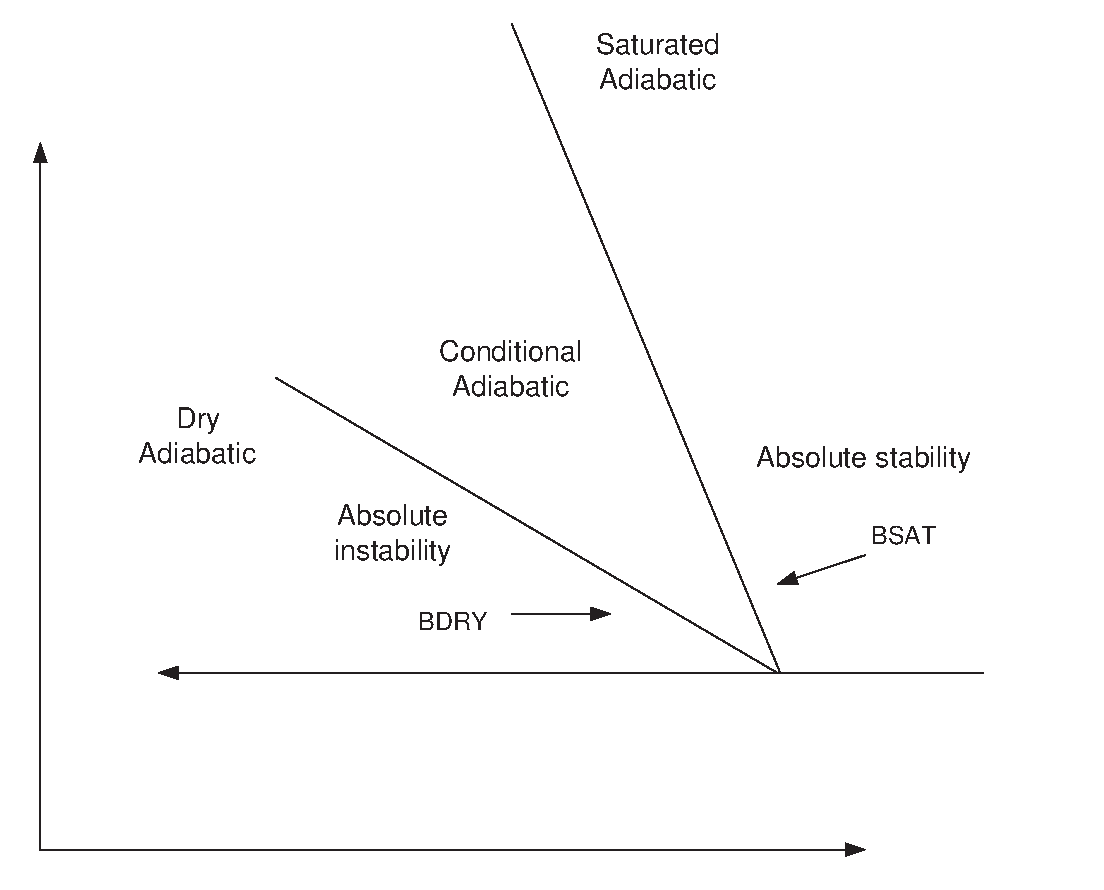
\includegraphics[width=11cm]{vertstab.eps}
    \caption{Stability conditions for the vertical stability of saturated and unsaturated air.} %this is how it shows up in the List of Figures
    \label{f:verticalstab}
    \end{figure}
.\\    
And finally I end this example file with a table which will be centered in the middle of the following page
\begin{table}[hp]
\centering
\renewcommand{\arraystretch}{1.5}
\begin{tabular}{|ll|}
\hline
\multicolumn{2}{|c|}{\bf\sffamily {\it Data} files listed in a table }\\
\hline\hline
\multicolumn{2}{|l|}{\bf\sffamily First part} \\
Fabracadabra.m	& - Saturation computation\\
Fobracadabra.m	& - Pressure computation\\
Fibricadibri.m	& - Permeability computation\\
&\\
\multicolumn{2}{|l|}{\bf\sffamily Structural rock model} \\
struct.m	& - Rock structural data using symmetric boundary condition \\
bstruct.m	& - Rock structural data using anti-symmetric boundary condition \\
\hline
\end{tabular}
\caption{Good-looking program data deck files.} %this is how it shows up in the List of Tables
\label{tbl:tbl}
\end{table}
